Here I am talking about the raster and how friggin awesome it is.

\begin{figure}
	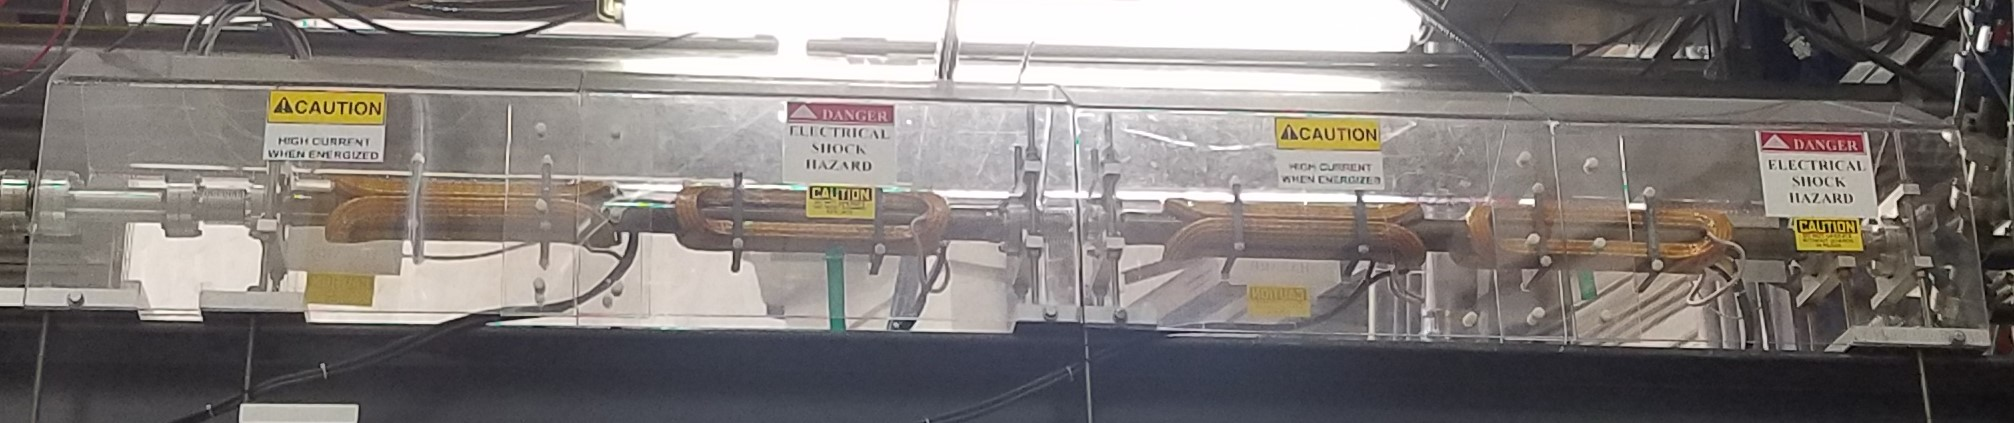
\includegraphics[width=\linewidth]{./chap2-exp/fig/raster_pic.jpg}
	\caption{The Hall A raster consists of four dipole magnets on the beamline}
	\label{fig:raster}
\end{figure}

The raster is a beamline apparatus in Hall A for spreading the beam onto the target, rather than being at a single point. This is done to prevent localized heating of the target. The raster consists of four dipole magnets, two for steering in the x-direction and two for steering in the y-direction.

Each raster magnet is powered by a triangle wave of approximately 25kHz. \textbf{When running properly, the x-direction magnets will be synced and the y-direction magnets will be synced. FIX SENTENCE FOR REDUNDANCY.} This syncing ensures that the magnets are always working together to create the desired beam spread.

\begin{figure}
	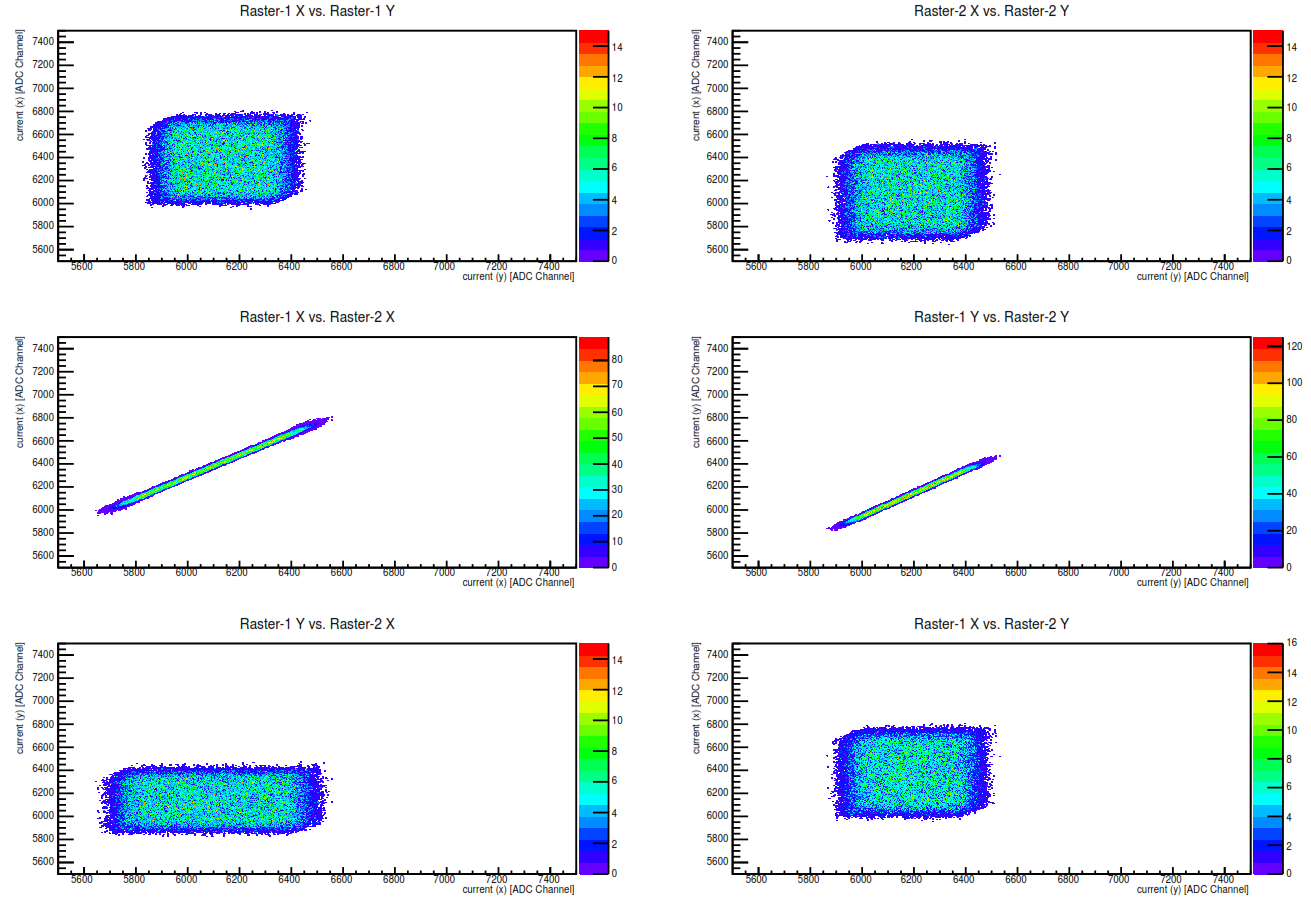
\includegraphics[width=\linewidth]{./chap2-exp/fig/raster_sync.png}
	\caption{The X and Y raster pairs are each synced to produce the maximum kick. The X and Y directions are uncorrelated so that the beam travels uniformly over the target.}
	\label{fig:raster}
\end{figure}